\nonstopmode
\documentclass[10pt, a4paper]{article}
%\usepackage{subfig}

\parindent=20pt
\parskip=8pt
\usepackage[width=15.5cm, left=3cm, top=2.5cm, height= 24.5cm]{geometry}

\usepackage[spanish]{babel}
\usepackage[utf8]{inputenc}
\usepackage{fancyhdr}
\usepackage{indentfirst}
\usepackage{latexsym}
\usepackage{caratula}
\usepackage{gnuplottex}
\usepackage{lastpage}
\usepackage{amsfonts}
\usepackage{listings}
\usepackage{pdfpages}
\lstset{language=C}
\usepackage[ruled,vlined,linesnumbered]{algorithm2e}
\usepackage{graphicx}
\usepackage{float}
\usepackage{color}

\graphicspath{{imgs/}}



% Acomodo fancyhdr.
\pagestyle{fancy}
\thispagestyle{fancy}
\addtolength{\headheight}{1pt}
\lhead{Algoritmos y Estructuras de Datos 3}
\rhead{TP1}
\cfoot{\thepage /\pageref{LastPage}}
\renewcommand{\footrulewidth}{0.4pt}
\renewcommand{\thesubsubsection}{\thesubsection.\alph{subsubsection}}




\author{Algoritmos y Estructuras de Datos III, DC, UBA.}
\date{}
\title{}

\begin{document}
	
\thispagestyle{empty}
\materia{Algoritmos y Estructuras de Datos III}
\submateria{Trabajo Pr\'actico N$^{\circ}$1}
\titulo{}
\integrante{Izcovich, Sabrina}{550/11}{sizcovich@gmail.com}
\integrante{Garcia Marset, Matias}{356/11}{matiasgarciamarset@gmail.com}
\integrante{Orellana, Ignacio}{229/11}{nacho@foxdev.com.ar}
\integrante{Vita, Sebastián}{149/11}{sebastian\_vita@yahoo.com.ar}

\maketitle

\tableofcontents
\newpage

\section{Introducci\'on}
Este trabajo práctico consiste en la resolución de ciertos problemas algorítmicos que cumplen con restricciones impuestas por la cátedra, como por ejemplo el orden de complejidad máximo de los mismos, entre otras. Para justificar las implementaciones de los problemas en cuestión, fue necesaria la utilización de herramientas lógico-matemáticas que serán mencionadas a lo largo del desarrollo de cada ejercicio.\newline
Para comprobar que nuestras soluciones resolvieran correctamente los problemas propuestos, debimos dividir el análisis de los mismos en secciones a fin de estudiar minuciosamente las características de éstos. Estas secciones se dividen de la siguiente forma:\newline

\begin{itemize}
\item \textbf{Problema a resolver:} En esta sección, nos encargamos de describir detalladamente el problema a resolver dando ejemplos del mismo y sus soluciones.
\item \textbf{Resolución coloquial:} En esta parte, nos dedicamos a explicar de forma clara, sencilla, estructurada y concisa las ideas desarrolladas para la resolución del problema en cuestión. Para ello, decidimos utilizar pseudocódigo y lenguaje coloquial combinando ambas herramientas de manera adecuada.
\item \textbf{Demostración de correctitud:} Utilizamos este apartado para justificar que el punto anterior resuelve efectivamente el problema y demostramos formalmente la correctitud del mismo.
\item \textbf{Complejidad del algoritmo:} En esta sección, nos ocupamos de deducir una cota de complejidad temporal del algoritmo propuesto en función de los parámetros considerados como correctos. Por otro lado, justificamos por qué el algoritmo desarrollado para la resolución del problema cumple con la cota dada.
\item \textbf{Código fuente:} En esta parte, presentamos las funciones relevantes del código fuente que implementa la solución propuesta. Para ello, decidimos utilizar el lenguaje \verb*#C++# dado que éste cuenta con la librería $stl$ que proporciona las estructuras necesarias para la realización de dicha tarea.
\item \textbf{Instancias posibles:} Este sector presenta un conjunto de instancias que permiten verificar la correctitud del programa implementado cubriendo todos los casos posibles y justificando la elección de los mismos. Dichas instancias fueron evaluadas por el algoritmo realizado y los resultados obtenidos fueron comprobados.
\item \textbf{Testing:} Por último, los tests consistieron en experimentaciones computacionales utilizadas para medir la performance del programa implementado. Para ello, debimos preparar un conjunto de casos de test que permitieran observar los tiempos de ejecución en función de los parámetros de entrada que fueran relevantes. Para ello, nos encargamos de generar instancias aleatorias como también particulares. Para que los resultados fueran visibles y claros, utilizamos una comparación gráfica entre los tiempos medidos y la complejidad teórica calculada.
\end{itemize}
\newpage

\section{Ejercicio 1}
\subsection{Problema a resolver}
El siguiente ejercicio consiste en hallar una manera de implementar un sistema proporcionado respetando una cota determinada de orden de complejidad. El problema se sitúa en un centro de distribución de correo que recibe paquetes todos los días cuyo destino final es la sede central de la empresa. Para el transporte de los mismos, éstos son cargados a camiones de igual capacidad. El encargado de logística, Pascual, tiene un sistema que utiliza desde hace años para agilizar la carga de los camiones asegurando el uso de una baja cantidad de los mismos para el envío de paquetes al final del día. Dicho sistema consiste en agarrar los paquetes y ubicarlos en algún camión que ya tenga paquetes dentro, eligiendo entre éstos el que menos peso esté cargando hasta ese momento. Si el peso del paquete permite que éste sea cargado en ese camión, se lo ubica allí, sino, se lo incluye en un nuevo camión.\newline
El problema a resolver se basa en escribir un algoritmo que tome los pesos de los paquetes que hay que acomodar e indique cuántos camiones se van a utilizar y cuánto peso se cargará en cada uno de ellos al final del día considerando el sistema de Pascual. Para esto, se respeta el orden de llegada de los paquetes a medida que ingresan. \newline
Las consideraciones a tener en cuenta son que los camiones tienen la misma capacidad de carga, la cantidad disponible de los mismos alcanza para transportar todos los paquetes y que el peso de un paquete no supera la capacidad de carga de un camión. Del mismo modo, el tamaño de los paquetes no es tenido en cuenta. Además, es importante tener en cuenta que las cargas son valores enteros positivos.\newline
\newline
\textbf {Formatos de entrada y salida:}\newline
\newline
La entrada contiene varias instancias del problema. Cada instancia consta de una línea con el siguiente formato:

$$L\ n\ p_{1}\ p_{2}\ ...\ p_{n}$$


donde \textbf{$L$} es el límite de carga de los camiones, \textbf{$n$} es la cantidad de paquetes a acomodar y \textbf{$p_{1}$, ..., $p_{n}$} son los pesos de cada paquete en el orden en el que deben ser almacenados.\newline

La salida debe contener una línea por cada instancia de entrada, con el siguiente formato:

$$k\ c_{1}\ c_{2}\ ...\ c_{n}$$


donde \textbf{$k$} es la cantidad de camiones utilizados y \textbf{$c_{1}$, ..., $c_{k}$} es el peso que se cargó en cada uno de los \textbf{$k$} camiones al final del día.\newline

En lo que sigue, presentaremos dos ejemplos sobre el sistema impulsado por Pascual:
\begin{itemize}
\item {\large{\textbf{Ejemplo 1:}}}\newline

En este ejemplo, decidimos conveniente develar un caso en el que fuera agregado un paquete a un camión ya cargado. Por otro lado, quisimos contrarestarlo insertando un paquete con una carga que superaba la capacidad del camión creado anteriormente. Por último, nos pareció importante mostrar un caso en el que al agregar un nuevo paquete, si bien un nuevo camión había sido creado, éste era colocado en el camión cuya carga fuera la menor.\newline

\textbf{Formato de entrada:}
$$100\ \ 5\ \ 20\ \ 40\ \ 80\ \ 15\ \ 100$$

\begin{figure}[H] %[h] Aqui [b] para button [t] para top
\begin{center}
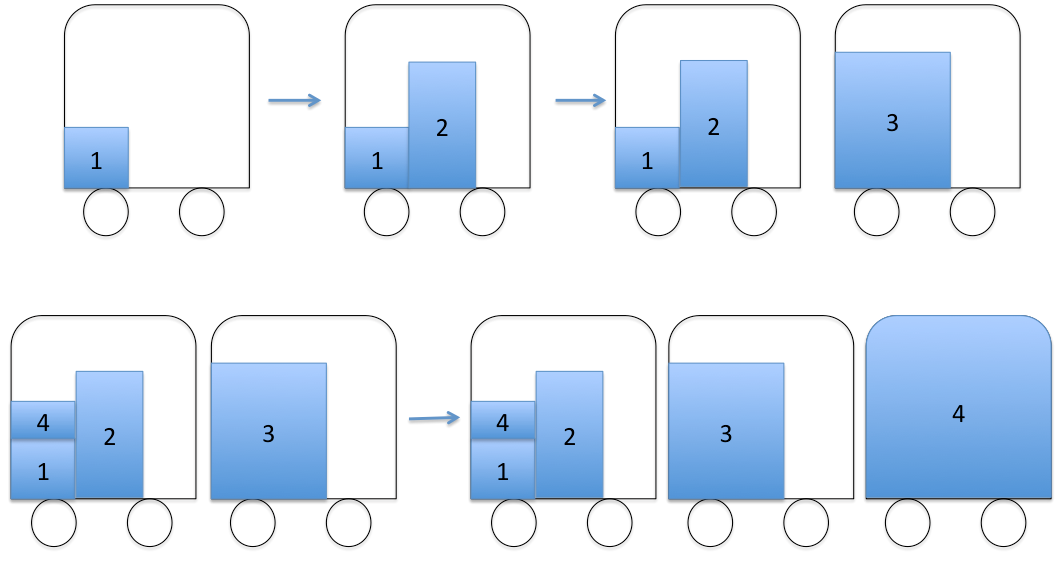
\includegraphics[width=320pt]{../imgs/ejemplo1.jpg}
\end{center}
\end{figure}

\textbf{Formato de salida:}
$$3\ \ 75\ \ 80\ \ 100$$


\item {\large{\textbf{Ejemplo 2:}}}\newline

En este ejemplo, quisimos mostrar lo que ocurría en caso en el que cada paquete superara el 50\% de la carga disponible en un camión.\newline

\textbf{Formato de entrada:} 
$$150\ \ 3\ \ 80\ \ 75\ \ 82$$

\begin{figure}[H] %[h] Aqui [b] para button [t] para top
\begin{center}
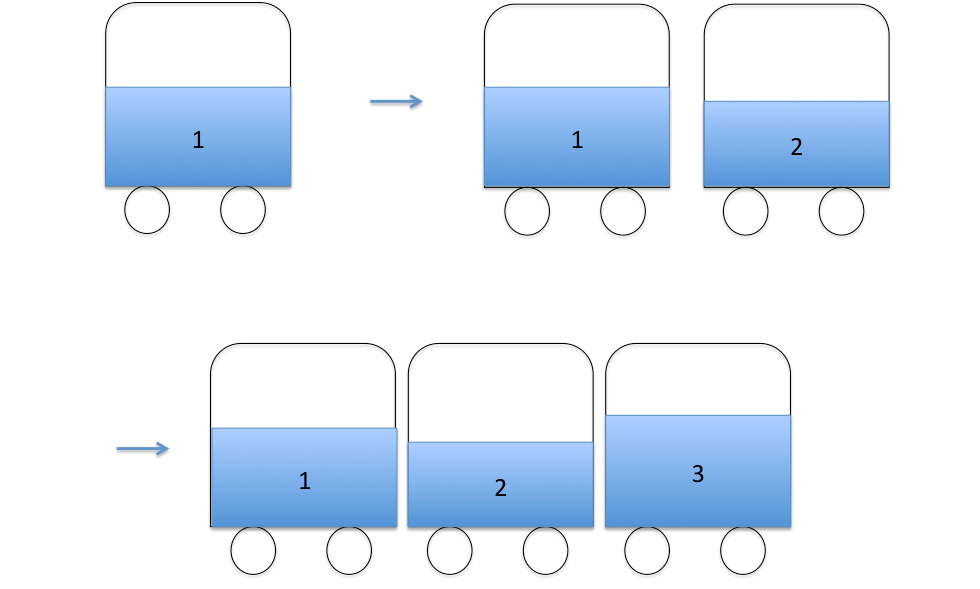
\includegraphics[width=300pt]{../imgs/ejemplo2.jpg}
\end{center}
\end{figure}

\textbf{Formato de salida:}
$$3\ \ 80\ \ 75\ \ 82$$


\end{itemize}
\subsection{Resolución coloquial}
Al analizar el problema a resolver, nos percatamos de que lo más conveniente era implementar la solución en base a un $algoritmo\ goloso$. Dicho algoritmo consiste en la construcción de una solución seleccionando, en cada paso, la mejor alternativa sin considerar las implicancias de ésta.\newline Por otro lado, dicha técnica de diseño algorítmico resulta fácil de implementar, suele ser eficiente y permite construir soluciones razonables.\newline
\newline
En este caso, la resolución basada en un algoritmo goloso nos permitió tomar cada instancia de la entrada y ubicarla en el lugar más conveniente en ese momento. Esto significa que dada la $i-ésima$ caja ingresada en un mismo día, ésta era ubicada en el camión que menor cargado se encontraba en el momento en el que se la agregaba. Para lograr esto, decidimos utilizar como estructura un heap.\newline
\newline
Un heap consiste en una estructura de datos del tipo árbol binario completo con información perteneciente a un tipo de datos cumpliendo con un cierto orden. Un heap máximo tiene la característica de que cada nodo padre tiene un valor mayor que el de cualquiera de sus nodos hijos.\newline
Para adaptar el problema de Pascual al heap, decidimos que cada nodo debía representar la capacidad de carga disponible correspondiente a un camión determinado en un momento dado.\newline
\newline
El pseudocódigo ideado para resolver el problema es el siguiente:\newline

\begin{algorithm}[H]
	\SetAlgoLined
	\caption{Algoritmo de Pascual}
	\KwIn{capacidadCamion, cantidadDePaquetes, pesosDePaquetes}
	\KwOut{cantidadDeCamiones, listaDeCamiones}
	cantidadDeCamiones = 0\\
	actual = 0\\
	camionesCreados = vacio\
	\While{pesosDePaquetes $\geq$ vacio}{
	\eIf{camionesCreados $\neq$ vacio $\land$ camionMenosCargado(camionesCreados)\footnote{Esta funcion devuelve el camion menos cargado} $\geq$ $pesosDePaquetes_{actual}$}{
		camionActual = camionMenosCargado(camionesCreados)\\
		camionActual = camionActual - $pesosDePaquetes_{actual}$\\
		camionesCreados $\leftarrow$ camionActual
		}{
			camionActual = capacidadCamion - $pesosDePaquetes_{actual}$	\\
			camionesCreados $\leftarrow$ camionActual\\
			cantidadDeCamiones = cantidadDeCamiones + 1\\
		}	
		actual = actual + 1\\
		
	}
\end{algorithm}

\begin{algorithm}[H]
	\SetAlgoLined
	\caption{Algoritmo de Pascual (version Nacho)}
	\KwIn{Paquetes $ps$}
	\KwOut{cantidadDeCamiones, listaDePesos}

	Camiones $ca \leftarrow \{nuevoCamion\}$\\
	cantidadDeCamiones := 0\\
	\lIf{$ps = \emptyset$}{\textbf{devolver} 0, $\emptyset$}\\
	\For{Paquete p $\in$ $ps$}{
		Camion $c$ := camionMenosCargado($ca$)\\
		\eIf{peso($p$) $\leq$ capacidad($c$)}{
			capacidad($c$) $-=$ peso($p$)
		}{
			$ca \leftarrow$ Camion $cNuevo$\\
			capacidad($cNuevo$) $-=$ peso($p$)
		}
	}
	\textbf{devolver} cantidadDeCamiones, $ca$


\end{algorithm}

\subsection{Demostración de correctitud}
Esta estructura resultó la más adecuada para nuestra implementación dado que 



\subsection{Complejidad del algoritmo}
Tal como requerido, la complejidad temporal del algoritmo debe ser estrictamente menor a $\mathcal{O}(n^2)$.


\subsection{Código fuente}



\subsection{Instancias posibles}



\subsection{Testing}

\newpage

\section{Ejercicio 2}
\subsection{Problema a resolver}
El siguiente ejercicio consiste en exponer un algoritmo capaz de devolver, dado un conjunto de intervalos, el subconjunto máximo de los que no se solapan entre sí. Dichos intervalos se conforman por una fecha de inicio $i$ y una de fin $f$. Luego, se pide que el resultado sea uno de los conjuntos $C$ de máximos intervalos posibles que cumpla con la siguiente propiedad: $$\forall v_{1}, v_{2} \in C, v_{1} \neq v_{2}\ | \ (f_{v_{1}} < i_{v_{2}}) \vee (f_{v_{2}} < i_{v_{1}}).$$ Luego, el algoritmo debe poder tomar las fechas ofrecidas por los profesores del programa de Profesores Visitantes de la FCEyN para sus cursos e indicar qué cursos deberían elegirse para maximizar la cantidad de éstos en el ciclo. Cada intervalo corresponde a la fecha en que un profesor dictará su curso. El primer elemento del intervalo corresponde a la fecha de inicio y el segundo a la fecha de fin, siendo siempre la de fin mayor o igual a la de inicio. Para la simplificación del manejo de los datos, éstos se representan con números enteros positivos.\newline
\newline
\textbf {Formatos de entrada y salida:}\newline
\newline
La entrada contiene varias instancias del problema. Cada instancia consta de una línea con el siguiente formato:

$$n\ i_{1}\ f_{1}\ i_{2}\ f_{2}\ ...\ i_{n}\ f_{n}$$


donde \textbf{$n$} es la cantidad de cursos ofrecidos por los profesores (numerados de 1 a n) y los valores \textbf{$[i_{1},f_{1}],\ ...,\ [i_{n},f_{n}]$} representan los días de inicio y fin de cada uno de los n cursos. Todos los datos son enteros positivos. La entrada concluye con una línea comenzada por \# que no debe ser procesada.\newline

La salida debe contener una línea por cada instancia de entrada, donde se listan los números de los cursos elegidos para el ciclo de cursos.\newline
\newline
En lo que sigue, presentaremos dos ejemplos sobre cómo debería comportarse nuestro algoritmo:\newline

{\large{\textbf{Ejemplos:}}}\newline

\begin{figure}[H] %[h] Aqui [b] para button [t] para top
\begin{center}
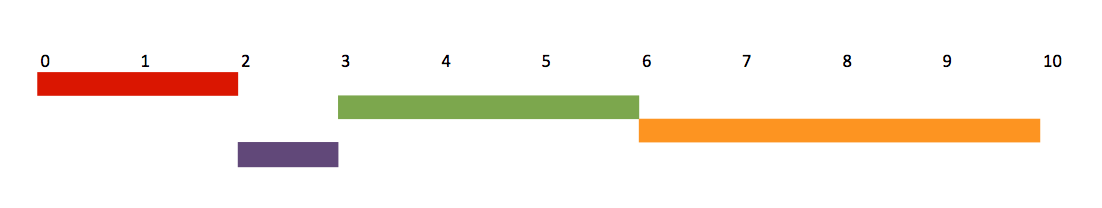
\includegraphics[width=460pt]{../imgs/ejemplo1ej2.png}
\end{center}
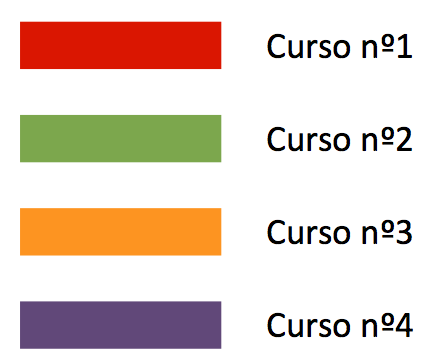
\includegraphics[width=90pt]{../imgs/leyendaej2.png}
\caption{Ejemplo 1.}
\end{figure}

\textbf{Formato de entrada:} $$4\ \ 0\ \ 1\ \ 2\ \ 2\ \ 3\ \ 5\ \ 6\ \ 9$$

\textbf{Formato de salida:} $$3\ \ 2\ \ 3\ \ 4$$


\begin{figure}[H] %[h] Aqui [b] para button [t] para top
\begin{center}
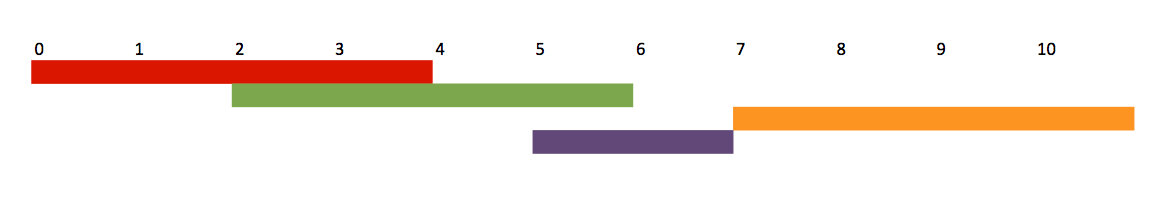
\includegraphics[width=480pt]{../imgs/ejemplo2ej2.png}
\end{center}
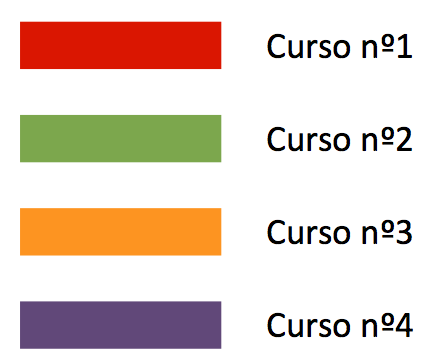
\includegraphics[width=90pt]{../imgs/leyendaej2.png}
\caption{Ejemplo 2.}
\end{figure}

\textbf{Formato de entrada:} $$4\ \ 0\ \ 3\ \ 2\ \ 5\ \ 5\ \ 6\ \ 7\ \ 10$$

\textbf{Formato de salida:} $$3\ \ 1\ \ 3\ \ 4$$



\subsection{Resolución coloquial}

Decidimos resolver el problema ordenando los cursos de acuerdo a la fecha de finalización de los mismos por orden creciente. De este modo, se recorrió cada intervalo correspondiente a cada curso y, cuando el $i-ésimo$ no se solapaba con el $i-ésimo\ -\ 1$, se lo agregaba a la solución.\newline
Al analizar el problema a resolver, nos percatamos de que el algoritmo de maximización de intervalos no solapados corresponde a un $algoritmo\ goloso$. El pseudocódigo que describe el algoritmo es el siguiente:\newline

\begin{algorithm}[H]
    \SetAlgoLined
    \caption{MaximaCantidadDeIntervalosNoSolapados}
    \KwIn{Cursos $CS$}
    \KwOut{listaDeCursos}
    Lista $seleccionados$ = lista de booleanos que representan si un curso fue elegido
    \eIf{\#CS == 0}{
        \textbf{devolver} $ListaVacia$\\
    }{
        $CS$ = OrdenarPorFin($CS$)\\
        filtrarSolapamientos($CS$, $seleccionados$)\\
        Lista $res$ = filtrar($seleccionado$)\\
        \textbf{devolver} \#res ++ res\\
    }
\end{algorithm}

\begin{algorithm}[H]
    \SetAlgoLined
    \caption{filtrarSolapamientos}
    \KwIn{Cursos $CS$}
    \KwOut{listaDeCursos}
    Curso $anterior$ = Primer curso de $CS$\\
    \For{Curso $c$ en $CS$}{
        \If{$c$ noSeSolapa con $anterior$}{
            $anterior$ := $c$\\
            $seleccionado_{c.indice} := true$
        }
    }
    \textbf{devolver} $res$\\   
\end{algorithm}


donde $Cursos$ es una secuencia conteniendo la información (fecha de inicio y de fin) de los cursos del ciclo, $ordenarPorFin$ es un algoritmo que toma los cursos y los ordena de acuerdo a su fecha de finalización y $noSeSolapa$ verifica que la fecha de inicio del intervalo que se quiere agregar no se superponga con la fecha de fin del agregado precedentemente. Por otro lado, $filtrar$ recorre la lista de $seleccionados$ y se queda con aquellos cuyo valor es $true$.

\subsection{Demostración de correctitud}

Veamos que, efectivamente, nuestro algoritmo encuentra una solución óptima $S$ cuya cantidad de intervalos es $k$. Para ello, vamos a suponer que tenemos la salida ordenada por la fecha de fin de cada intervalo. Supongamos que existe una solución óptima $S'$ cuya cantidad de intervalos es $n$, dicha solución se encuentra ordenada del mismo modo que $S$.\\
\newline
Sean $S_{1}$ y $S'_{1}$ los primeros intervalos de ambas soluciones. En el caso en el que $f_{S_{1}} \leq f_{S'_{1}}$, se puede reemplazar $S'_{1}$ por $S_{1}$ pues, si $S'_{2}$ no se solapa con $S'_{1}$, tampoco lo hará con $S_{1}$. El caso $f_{S'_{1}} < f_{S_{1}}$ no puede ocurrir pues nuestro algoritmo selecciona el intervalo cuya fecha de fin es la menor.\\
\newline
Por otra parte, si consideramos $S_{2}$ y $S'_{2}$ y por el mismo criterio utilizado anteriormente, si $f_{S_{2}} \leq f_{S'_{2}}$, se puede reemplazar $S'_{2}$ por $S_{2}$ pues, si $S'_{1}$ no se solapa con $S'_{2}$, tampoco se solapará con $S_{2}$. Este mismo razonamiento puede extenderse, con el mismo principio, hasta $S_{k}$.\\
\newline
Tal como mencionado, los intervalos de nuestra solución terminan igual o antes que los de la solución óptima, en particular, el último de ellos. Veamos ahora, qué relación existe entre $k$ y $n$. Para ello, analicemos las diferentes posibilidades:
\begin{itemize}
\item \textbf{$k = n$:} En este caso, la solución proporcionada por nuestro algoritmo tiene la misma cantidad de intervalos que la óptima. Luego, es óptimo.
\item \textbf{$k > n$:} Esta situación no es posible dado que $n$ es la cantidad de intervalos de la solución óptima por lo que $k \leq n$.
\item \textbf{$k < n$:} En este caso, existe un intervalo en $S'_{k+1}$ cuya fecha de fin es mayor a la fecha de fin de $S_{k}$ dado que éste reemplazó a $S'_{k}$. Pero esto resulta absurdo pues este intervalo debería estar también en $S$ como lo estipula nuestro algoritmo.
\end{itemize}

Luego, podemos concluir que $k = n$, siendo, la solución de nuestro algoritmo, la óptima al problema. 

\subsection{Complejidad del algoritmo}

Sea $n$ la cantidad de cursos del ciclo del programa de Profesores Visitantes de la FCEyN. Para analizar la complejidad de nuestro algoritmo, debemos tener en cuenta lo que sigue:
\begin{itemize}
\item La complejidad del algoritmo \textbf{Sort} es $\mathcal{O}(n\ log\ n)$\footnote{http://en.cppreference.com/w/cpp/algorithm/sort}.
\item La complejidad del \textbf{constructor} que utilizamos sobre la estructura \textbf{vector} es $\mathcal{O}(1)$\footnote{http://en.cppreference.com/w/cpp/container/vector/vector}.
\item La complejidad del algoritmo \textbf{push$\_$back} sobre la estructura \textbf{vector} es $\mathcal{O}(1)$ amortizado \footnote{http://en.cppreference.com/w/cpp/container/vector/push$\_$back}. 
\item La complejidad del algoritmo \textbf{size} sobre la estructura \textbf{vector} es $\mathcal{O}(1)$\footnote{http://en.cppreference.com/w/cpp/container/vector/size}.
\item La complejidad de la función \textbf{filtrarSolapamientos} recorre todos los cursos y, en cada paso, pregunta si se solapa el actual con el anterior. Dicha comparación resulta constante dado que es de enteros, y luego de ser asi, cambia una variable en un vector ya definido y se asigna una variable (todo esto en tiempo constante). Recorrer el for tiene un costo de complejidad lineal en el peor caso y no crece ya que lo que se hace adentro es constante.
\end{itemize}

Luego, al comienzo del algoritmo se ordena la lista de cursos, eso se hace con la función \textbf{sort} que tiene una complejidad de O($n*log\ n$) y luego se aplica \textbf{filtrarSolapamientos} que tiene una complejidad lineal, finalmente se devuelve el resultado, con lo cual la complejidad final es O($n*log\ n$) + O($n$) lo cual esta acotado asintóticamente por O($n*log\ n$), que es lo que queriamos ver.

\subsection{Código fuente}

\begin{figure}[H]
\begin{center}
\begin{verbatim}
if (cs.size() == 0) {
    res.push_back(0);
    return res;
} else {
    for (int i = 0; i < cs.size(); ++i)
        seleccionados.push_back(false);
    sort(cs.begin(), cs.end(),customLess);
    filtrarSolapamientos();
    res.push_back(cantSeleccionados);
    for (int i = 0; i < seleccionados.size(); ++i)
        if (seleccionados[i])
            res.push_back(i+1);
    return res;
}
\end{verbatim}
\caption{Codigo de ejercicio 1}
\end{center}
\end{figure}

\begin{figure}[H]
\begin{center}
\begin{verbatim}
for(int i = 1; i < cs.size(); ++i) {
    if (cs[i].second.first > anterior.second.second) {
        anterior = cs[i];
        seleccionados[cs[i].first] = true;
        cantSeleccionados++;
    }
}
\end{verbatim}
\caption{Codigo de filtrarSolapamientos}
\end{center}
\end{figure}



\{Instancias posibles}

Para verificar la correctitud de nuestro programa, dispusimos variar estratégicamente las instancias de entrada al ejecutarlo.
\begin{itemize}
\item En primer lugar, decidimos mostrar un caso en el que no se solapara ningún curso. En esta ocasión, puede observarse que, dado que hay una solución óptima, ésta es única. De este modo, se logra verificar que los cursos de la entrada coinciden con los de la salida.\newline
\textbf{Parámetro de entrada:} $$3\ \ 0\ \ 1\ \ 3\ \ 5\ \ 6\ \ 9$$
\textbf{Parámetro de salida:} $$3\ \ 1\ \ 2\ \ 3$$\newline


\begin{figure}[H] %[h] Aqui [b] para button [t] para top
\begin{center}
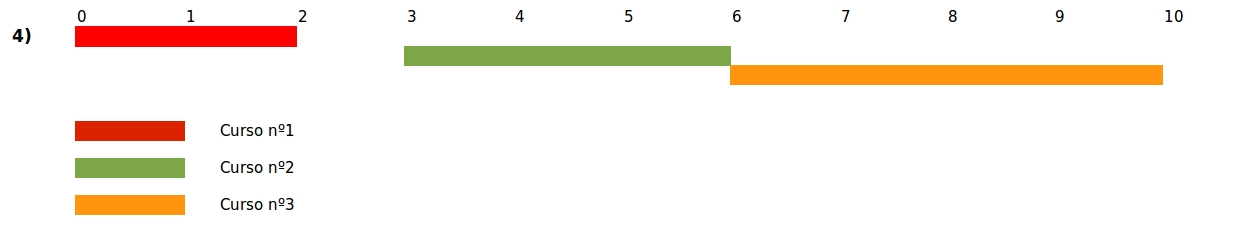
\includegraphics[width=450pt]{../imgs/instancia4.jpg}
\end{center}
\caption{Instancia posible nº1.}
\end{figure}

\item Por otra parte, probamos el programa para la situación en la que no se ingresa ningún curso. Esto sería, por lo tanto, el caso vacío. Dado que este caso borde es muy significativo, nos pareció interesante mencionarlo.\newline
\textbf{Parámetro de entrada:} $$0$$
\textbf{Parámetro de salida:} $$0$$ \newline


\item Otro caso a considerar es en el que todos los cursos finalizan el mismo día (solapándose todos entre sí). Debido a que cualquiera de ellos es solución del problema pues es la máxima cantidad de intervalos que no se solapan, utilizamos esta instancia para verificar que nuestro algoritmo devolviera siempre el de menor fecha de finalización. \newline
\textbf{Parámetro de entrada:}  $$3\ \ 1\ \ 5\ \ 3\ \ 5\ \ 2\ \ 5$$
\textbf{Parámetro de salida:}  $$1\ \ 1$$\newline

\begin{figure}[H] %[h] Aqui [b] para button [t] para top
\begin{center}
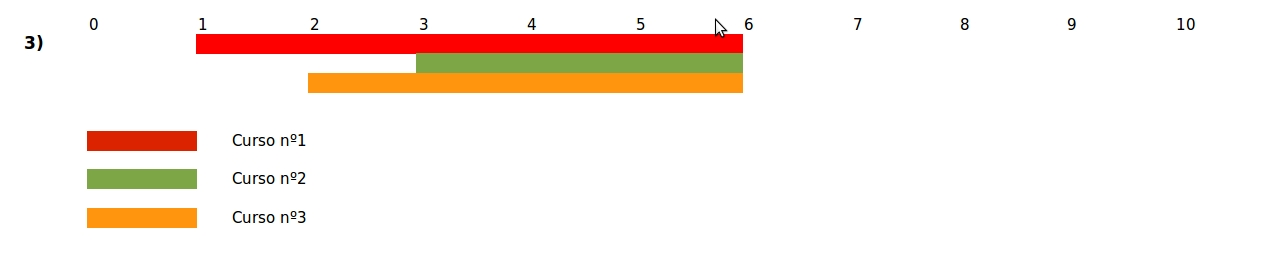
\includegraphics[width=450pt]{../imgs/instancia3.jpg}
\end{center}
\caption{Instancia posible nº3.}
\end{figure}


\item Por último, consideramos interesante considerar el caso en el que existe al menos un curso que se solapa. Dicho caso sería el más común en el problema a resolver. Este tipo de situaciones tienen más de una solución óptima. En esta oportunidad, hay dos salidas posibles que son solución del problema. Debido que nuestro algoritmo almacena, en primer lugar, los intervalos cuya fecha de fin es la más alta, dicho intervalo es el prioritario frente a cualquiera que se le solape. Del mismo modo, decidimos que podía ser interesante considerar el caso de cursos cuya fecha de inicio fuera igual a la fecha de fin para comprobar que las cotas del programa estuvieran definidas correctamente.\newline
\textbf{Parámetro de entrada:}  $$4\ \ 0\ \ 3\ \ 3\ \ 5\ \ 7\ \ 10\ \ 8\ \ 9$$
\textbf{Parámetro de salida:}  $$2\ \ 1\ \ 4$$ \newline

\begin{figure}[H] %[h] Aqui [b] para button [t] para top
\begin{center}
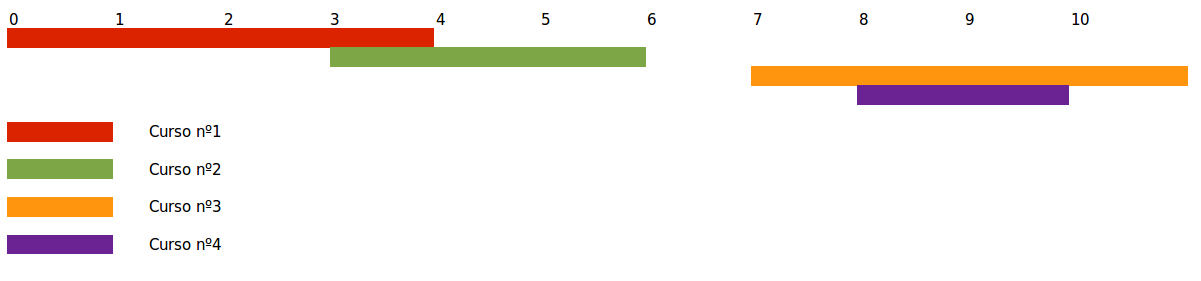
\includegraphics[width=450pt]{../imgs/instancia1.jpg}
\end{center}
\caption{Instancia posible nº4.}
\end{figure}

\end{itemize}

\subsection{Testing}

\newpage

\section{Ejercicio 3}
\subsection{Problema a resolver}

\subsection{Resolución coloquial}

\subsection{Demostración de correctitud}

\subsection{Complejidad del algoritmo}

\subsection{Código fuente}

\subsection{Instancias posibles}

\subsection{Testing}

\newpage

\section{Referencias}

\begin{itemize}
\item http://dacap.com.ar/blog/cpp/cola-de-prioridades-stl-priority-queue/

\item https://www.lsi.upc.edu/ps/downloads/matdoc/transparencias/ps/ps\_VI\_heaps.pdf
\end{itemize}

\end{document}
